% !TEX root = ../main.tex

\section{Evaluating Proposed Solutions}\label{sec:eval}

In this section, we evaluate 10 solutions that have been proposed by Ethereum community---mostly from developers on GitHub---to address the multiple withdrawal attack. We examine each solution in detail and evaluate them against the criteria established in the previous section (see Section~\ref{sec:criteria}). The summary is presented in Figure~\ref{tab:comp}.

% = = = = = = = = = = = = = = = = = = = = = = = = = = = = = = = = = = = = = = = = = = =

\subsection{Enforcement by User Interface (UI)}
\label{sec:enfui}

\begin{figure}[t!]
	\centering
	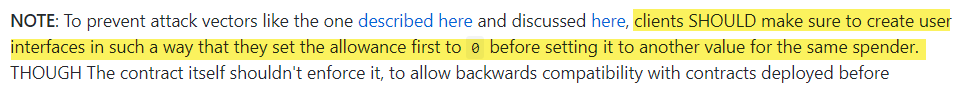
\includegraphics[width=1.0\linewidth]{figures/multiple_withdrawal_03.png}
	\caption{Recommendation of ERC20 standard to mitigate \textit{``multiple withdrawal attack''} by enforcement in UI.\label{fig:uie}}
\end{figure}

The first solution is enforcement at the user interface level. We discussed this previously in Section~\ref{sec:preho} but we reiterate the main points here again. The exact recommendation from the ERC20 standard is shown in Figure~\ref{fig:uie} and is essentially to set an allowance to zero before any non-zero values. Presumedly, it will also enforce that the new approval is not allowed if proceeded by a token transfer by the approved spender. We consider the UI to be a lightweight web app that can reference a contract's state variables and emitted events but does not maintain a full copy of the blockchain. Consider (again) the most basic attack sequence:

% Jeremy: Even with logging events, if Bob sends to Carol, then Alice won't necessarily pause before step 5

\begin{enumerate}
	\item Alice allows Bob to transfer N of Alice's tokens.
	\item Alice's client broadcasts an allowance of 0 for Bob.
	\item Bob broadcasts a competing transaction to transfer N of Alice’s tokens.
	\item Bob's transaction front-runs Alice's, is confirmed, and sets Bob’s allowance to 0 (from N).
	\item Alice’s transaction is confirmed and sets Bob’s allowance to 0 (from 0).
	\item Alice's client broadcasts an allowance of M for Bob.
	\item Alice’s second transaction is confirmed and sets Bob's allowance to M.
	\item Bob transfers M of Alice’s tokens for a total of N+M tokens.
\end{enumerate}

The key mitigation to this attack is for Alice's client to pause at step 6 and determine if a transaction sequence like 3\&4 has occurred or not. This cannot be determined by monitoring the integer that records Bob's allowance because it will be 0 regardless of whether steps 3\&4 occurred or not. 

It also cannot always be determined by monitoring the events emitted from the contract. Step 4 will log a transfer from Alice's address to Bob's address of N tokens. If no event is emitted, Alice can know for certain no transfer was made. However if an event is emitted, Alice must decide it was a transfer initiated by Bob or a transfer by someone else she has authorized. If she has not authorized anyone else, she can know for certain it was Bob. However if she has a busy account with multiple authorized spenders of her tokens, the event is not verbose enough to determine what happened. Importantly, it does not record who initiated the transfer, only who received the tokens, and these are not necessarily the same entity. Bob can send Alice's tokens to his accomplice Carol, or some other authorized spender can send Alice's tokens to Bob (which looks like Bob is attacking when he is not). Since a UI is automated and does not use human discretion, it cannot decide circumstantially whether something looks like an attack or not --- it must either specify exact rules, which it cannot do here because of the ambiguity of the events, or it can ask for Alice's human input which introduces usability issues. In conclusion, it is better for enforcement to happen at the contract level.

% = = = = = = = = = = = = = = = = = = = = = = = = = = = = = = = = = = = = = = = = = = =

\subsection{MiniMeToken}
\label{sec:MiniMeToken}

%\begin{comment}
%// To change the approve amount you first have to reduce the addresses`
%//  allowance to zero by calling `approve(_spender,0)` if it is not
%//  already 0 to mitigate the race condition described here:
%//  https://github.com/ethereum/EIPs/issues/20#issuecomment-263524729
%require((_amount == 0) || (allowed[msg.sender][_spender] == 0));
%\end{comment}

\begin{figure}[t]
	\centering
	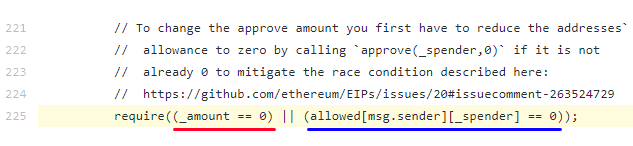
\includegraphics[width=1.0\linewidth]{figures/multiple_withdrawal_06.png}
	\caption{MiniMeToken added code to \texttt{approve} method for allowing non-zero allowance values if it is already set to zero.\label{fig:mini}}
\end{figure}

MiniMeToken~\cite{Ref15} enforces the recommendation that allowances are first set to zero before setting to a non-zero value. The enforcement is done within the ERC20 implementation itself by adding a check to the \texttt{approve} method (see Figure~\ref{fig:mini}). The red clause in line 225 (\texttt{\_amount == 0}) allows approvals to be set to 0, and the blue condition requires the allowance of \texttt{\_spender} to be 0 before it can be set to a non-zero value. This solution fails to prevent Bob from transferring N+M tokens, as the contract will be unable to determine whether N tokens have been already drained by Bob or not. Recall the attack sequence specified in the previous section (Section~\ref{fig:uie}). Step 5 will pass the red clause and Step 7 will pass the blue clause.

% Jeremy: We require it to be zero but don't know if it is zero because it was reset or because it was drained

% = = = = = = = = = = = = = = = = = = = = = = = = = = = = = = = = = = = = = = = = = = =

\subsection{MonolithDAO}
\label{sec:mdao}

\begin{figure}[t]
	\centering
	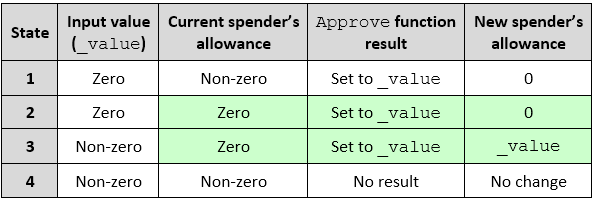
\includegraphics[width=1.0\linewidth]{figures/multiple_withdrawal_09.png}
	\caption{Functionality of the \texttt{approve} method in MiniMeToken and MonolithDAO tokens, which are implemented slightly differently but effectively enforce setting spender's allowance in two steps: first to zero and then to any non-zero value (\eg N$\rightarrow$0$\rightarrow$M).\label{fig:dao}}
\end{figure}

MonolithDAO Token~\cite{Ref12} (and its extension in OpenZeppelin~\cite{Ref10}) implement two additional functions for allowance increases and decreases: \texttt{increaseApproval} and \texttt{decreaseApproval}. Both take two parameters: the address of the approved spender and the amount to be added/subtracted from the spender's current approval. Additionally, the \texttt{approve} method is ERC20 compliant but has additional logic to enforce that owners either set the allowance to zero before non-zero values (see Figure~\ref{fig:dao}) or they use \texttt{decreaseApproval} and \texttt{increaseApproval} instead of \texttt{approve}. Forcing a set to zero is enforced the same way as in MiniMeToken~\ref{sec:MiniMeToken}). Consider the following transaction sequence:

\begin{enumerate}
	\item Alice allows Bob to transfer N of Alice's tokens by broadcasting \texttt{approve(\_Bob, N)}. 
	\item Remark: Alice can use the default \texttt{approve} method since Bob’s allowance was initially 0.
	\item Alice increases Bob’s allowance to M. \texttt{approve(\_Bob, M)} will fail because Bob's allowance is non-zero. Alice broadcasts \texttt{increaseApproval(\_Bob, M-N)}.
	\item Bob front-runs this by broadcasting \texttt{transferFrom(\_Alice, \_Bob, N)}.
	\item If Bob's transaction is confirmed first, he will transfer N tokens but this is legitimate as he was approved for N, and his approval is set to 0.
	\item Alice's transaction will adjust Bob's approval from 0 to M-N. In total, Bob can spend N+M-N = M tokens as intended.
	\item Remark: for decreases, decreaseApproval will similarly prevent the attack by reducing Bob's allowance instead of setting it to a particular value.
\end{enumerate}

Although these two new complementary functions do prevent the attack, they have not been defined in the initial specifications of ERC20 standard. Therefore, these safer functions will not be used by ERC20-compliant web apps and smart contracts that are already deployed. Such deployments will continue to use \texttt{approve} which suffers the same issue as MiniMeToken: set to zero does not always mitigate the attack. 

% Jeremy: I guess below means that someone just passes the approve parameters to the other function but I doubt anyone would blindly do that so removing it for now
%For example, if Alice has approved Bob for 100 tokens and wants to set it to 80, the new allowance should be 80 while using decrease methods will set it to 20 (100 - 80 = 20). Comparatively, increase method sets new allowance to 180 while it has to set it to 80 again to be in-compliant with ERC20 specification.

% = = = = = = = = = = = = = = = = = = = = = = = = = = = = = = = = = = = = = = = = = = =

\subsection{Detecting token transfers}

\begin{figure}[t]
	\centering
	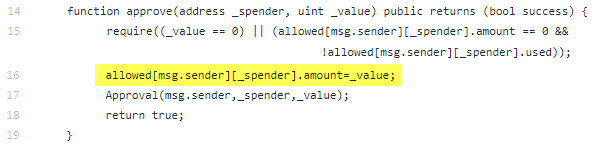
\includegraphics[width=1.0\linewidth]{figures/multiple_withdrawal_33.png}
	\caption{Detecting token transfers: \texttt{approve} method needs to be modified by adding a line of code like \texttt{allowed[msg.sender][\_spender].used = false;} between lines 16 and 17 to unlock spender flag for the next legitimate change. However, this change makes attack mitigation ineffective.\label{fig:det}}
\end{figure}

The next approach \cite{Ref17} maintains a small state machine to enforce prevent approvals preceded by transfers. We revisit and elaborate on this approach in our own solution in Section~\ref{sec:proposal1}. In this proposal, the implementation of \texttt{approve} is augmented with a flag (one flag for each pair of owners and approved spenders) that can be set in \texttt{transferFrom}. \texttt{transferFrom} sets the flag to \texttt{true} after any token transfer and the \texttt{approve} method requires the flag to be \texttt{false} before allowing new approvals. This approach requires a new data structure, can prevent front-running, but also has a deadlock scenario. Consider the following transaction sequence:

\begin{enumerate}
	\item Alice allows Bob to transfer N of Alice's tokens by broadcasting \texttt{approve(\_Bob, N)}. 
	\item Remark: This succeeds because Bob’s allowance was initially 0 and his corresponding flag=\texttt{false} (see line 16 in Figure~\ref{fig:det}).
	\item Alice decreases Bob's allowance to 0 by broadcasting \texttt{approve(\_Bob, 0)}.
	\item Bob front-runs this by broadcasting \texttt{transferFrom(\_Alice, \_Bob, N)}.
	\item If Bob's transaction is confirmed first, Bob's \texttt{transferFrom} turns his flag to \texttt{true}.
	\item Alice’s transaction is confirmed, passes the check because passed value is 0 (line 15), and Bob’s allowance is set to 0 while his flag remains \texttt{true}.
	\item Remark: Critically the \texttt{approve} method does not flip the spender's flag.
	\item Alice wants to change Bob’s allowance to M and broadcasts \texttt{approve(\_Bob, M)}. 
	\item Since Bob already transferred N tokens and his flag=\texttt{true}, the transaction fails.
	\item Remark: Bob’s allowance is 0 and it cannot not change so he is locked out of further approvals.
\end{enumerate}

%function approve(address _spender, uint _value) public returns (bool success) {
%	require((_value == 0) || (allowed[msg.sender][_spender].amount == 0 && !allowed[msg.sender][_spender].used));
%	allowed[msg.sender][_spender].amount=_value;
%	Approval(msg.sender,_spender,_value);
%	return true;
%}

Although this approach mitigates the attack, it prevents any further legitimate approvals. Consider a scenario where Alice wants to increase Bob’s allowance from N to M (two non-zero values). If Bob has already transferred number of tokens, Alice would not be able to change his approval. Because Bob's flag is set to \texttt{true} and line 15 in Figure~\ref{fig:det} does not allow changing the allowance, an exception is thrown. A potential bypass is to set the allowance to 0 and then to M. However this transaction sequence never flips the flag to \texttt{false} (there is no code for it in the \texttt{approve} method). So it keeps Bob locked out of any further legitimate allowances. A quick fix might be having \texttt{approve} set the flag to \texttt{false} (\ie between lines 16 and 17). But this will cause another problem: after setting the allowance to 0, the spender flag becomes \texttt{false}, and allows non-zero values even if tokens have been already transferred. This will no longer prevent multiple withdrawals as demonstrated in the following transaction sequence:

\begin{enumerate}
	\item Alice changes Bob's allowance from N to 0.
	\item Bob transfers N tokens before the allowance change and his \texttt{used} flag turns to \texttt{true}.
	\item Alice's transaction is successful since \texttt{\_value=0}. 
	\item Remark: The second condition is not evaluated although \texttt{used} flag is \texttt{true}.
	\item Alice's transaction turns \texttt{used} flag to \texttt{false} and sets Bob's allowance to 0. 
	\item Now Alice wants to set Bob's allowance from 0 to M, his flag is \texttt{false} and allowance is 0. 
	\item Remark: Alice cannot distinguish whether Bob moved any token or not. Setting a new allowance will allow Bob to transfer more tokens than Alice wanted.
\end{enumerate}

In fact, resetting the flag in \texttt{approve} method will not fix the issue and makes attack mitigation ineffective. In short, this approach can not satisfy both legitimate and non-legitimate scenarios. Nevertheless, it is a step forward by introducing the need for a new state to track transferred tokens if a solution is to be found.

% = = = = = = = = = = = = = = = = = = = = = = = = = = = = = = = = = = = = = = = = = = =

\subsection{Keeping track of remaining tokens}

\begin{figure}[t]
	\centering
	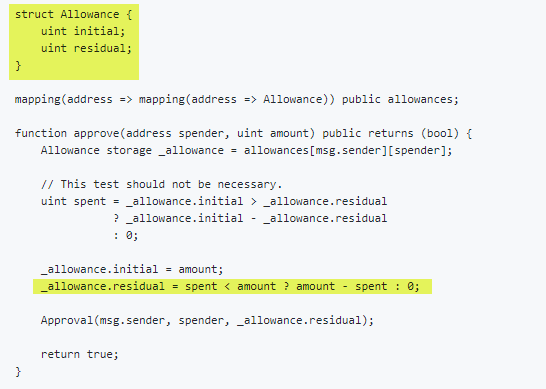
\includegraphics[width=1.0\linewidth]{figures/multiple_withdrawal_29.png}
	\caption{Keeping track of remaining tokens by introducing a new data structure.\label{fig:track}}
\end{figure}

This approach~\cite{Ref18} is inspired by the previous solution of detecting token transfers by introducing new state in the contract. It keeps track of the remaining tokens, and an ERC20-compliant \texttt{approve} method uses these variables to set allowances accordingly (see Figure~\ref{fig:track}).

%struct Allowance {
%	uint initial;
%	uint residual;
%}
%
%mapping(address => mapping(address => Allowance)) public allowances;
%
%function approve(address spender, uint amount) public returns (bool) {
%	Allowance storage _allowance = allowances[msg.sender][spender];
%	
%	// This test should not be necessary.
%	uint spent = _allowance.initial > _allowance.residual
%	? _allowance.initial - _allowance.residual
%	: 0;
%	
%	_allowance.initial = amount;
%	_allowance.residual = spent < amount ? amount - spent : 0;
%	
%	Approval(msg.sender, spender, _allowance.residual);
%	
%	return true;
%}
%
%function allowance(address holder, address spender) public view returns (uint) {
%	return allowances[holder][spender].residual;
%}
%
%function transferFrom(address holder, uint amount) public returns (bool) {
%	uint residual = allowance(holder, msg.sender);
%	
%	require(amount <= residual);
%	
%	allowances[holder][msg.sender].residual = residual - amount;
%	
%	// ... do the token transfer
%	
%	return true;
%}

At a first glance, it seems to be a promising solution by more effectively enforcing approvals to zero before non-zero values. However, the highlighted code in \texttt{approve} method resembles the situation that is explained in~\ref{sec:enfui}. In case of front-running, both \texttt{initial} and \texttt{residual} variables will be zero and it would not be possible for Alice to distinguish if any token transfer have occurred due to her allowance change or due to Bob transferring a token. To illustrate this, considering the following transaction sequence:

\begin{enumerate}
	\item Remark: For formatting reasons, we abbreviate \texttt{allowances[\_Alice][\_Bob].initial} as \texttt{AB.initial}.
	\item Bob’s allowance is initially zero (\texttt{AB.initial=0}) and his residual is zero as well (\texttt{AB.residual=0}).
	\item Alice allows Bob to transfer N tokens and makes \texttt{AB.initial=N} and \texttt{AB.residual=N}.
	\item Alice decides to change Bob’s allowance to M and has to set it to zero before M.
	\item Bob notices Alice’s broadcast for setting his allowance to 0 and frontruns it with a transfer of N tokens.
	\item Consequently, the \texttt{transferFrom} function sets his residual to zero (\texttt{AB.residual=0}).
	\item Alice’s transaction for setting Bob's allowance to 0 is confirmed and sets \texttt{AB.initial=0} and \texttt{AB.residual=0}.
	\item Remark: at this stage, the state is indistinguishable from Step 2. Alice cannot distinguish whether any token have been transferred or not based on \texttt{AB.initial} and \texttt{AB.residual}. 
	\item Alice approves Bob for spending new M tokens and Bob is able to transfer new M tokes in addition to initial N tokens.
\end{enumerate}

It is true that at Step 8, a transfer event as been recorded as a result of step 5. However transfer events are ambiguous as described in Section~\ref{sec:enfui}. Thus it is not always possible for the approver to detect legitimate from non-legitimate tokens transfers. Overall, this approach cannot prevent the attack in all scenarios. 

% = = = = = = = = = = = = = = = = = = = = = = = = = = = = = = = = = = = = = = = = = = =

\subsection{Overloading Approve}
\label{sec:overload}

% Jeremy: used to be
%\subsection{Changing the ERC20 API}

\begin{figure}[t]
	\centering
	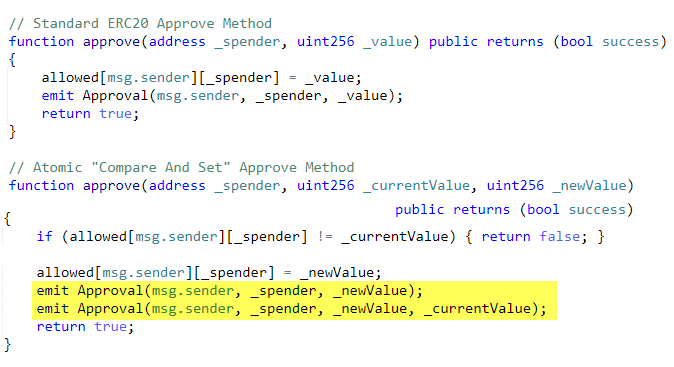
\includegraphics[width=1.0\linewidth]{figures/multiple_withdrawal_12.png}
	\caption{An overloaded approve method adds a method with three parameters to compare and set new allowance atomically.\label{fig:api}}
\end{figure}

As advised by \cite{Ref03}, a secure \texttt{approve} method could take one additional parameter: the expected allowance of the spender when the adjustment to the approval is made. Under this proposal, the adjustment succeeds only if the passed expected allowance matches the spender's actual allowance, and fails otherwise. Consider a multiple withdrawal attack where Bob is approved for N of Alice's tokens, Alice adjusts his approval from N to M tokens, and Bob frontruns the approval with a transfer of N tokens. Alice's approval will specify N as the current expected allowance when adjusting it to M. Because Bob's transfer of N tokens changes his approval to 0, Alice's approval will fail because it expects an allowance of N when the allowance is 0. This allows atomic compare and set of the spender's allowance to make the attack impossible. 

While this approach mitigates the attack, it requires a new overloaded \texttt{approve} method with three parameters, in addition to the standard ERC20 \texttt{approve} method with two parameters (see Figure~\ref{fig:api}). Additionally it defines a new event. Existing ERC20 web apps and smart contracts will be unaware of the overloaded method and continue to call the insecure two parameter method. Thus it does not provide interoperability. 

% Jeremy: I don't think this is true:
% Moreover, one more call is required to read current allowance and pass it to the new \texttt{approve} method.
% This can be executed without confirming to the blockchain

% = = = = = = = = = = = = = = = = = = = = = = = = = = = = = = = = = = = = = = = = = = =

\subsection{Alternate approval function}

Another suggestion \cite{Ref16} is to move the security check to a new function called \texttt{safeApprove}\footnote{\texttt{safeApprove(address \_spender, uint256 \_currentValue, uint256 \_value}} that compares the current and new allowance values (like the overloaded \texttt{approve} in Section~\ref{sec:overload}). The adjustment is only allowed if the allowance has not been changed by the time the function is executed. In this case, Alice uses the standard \texttt{approve} function to set Bob’s allowance to 0 and for new approvals, she has to use \texttt{safeApprove} function. As above, \texttt{safeApprove} takes the current expected approval amount as input parameter and calls \texttt{approve} method if previous allowance is equal to the current expected approval. Although this approach mitigates the attack by using the CAS pattern~\cite{Ref06}, it is not interoperable with ERC20-compliant web apps and smart contracts that will be unaware of \texttt{safeApprove}.

% = = = = = = = = = = = = = = = = = = = = = = = = = = = = = = = = = = = = = = = = = = =

\subsection{Minimum viable token}

Rather than adding new methods to ERC20, methods can be also be taken away. As suggested by the Ethereum Foundation\cite{Ref05}, we can reduce the ERC20 standard to a set of core functionalities and implement only the essential methods. The attack can be side-stepped if methods like \texttt{approve} and \texttt{transferFrom} are simply not implemented (recall that \texttt{transferFrom} is in addition to the more commonly used \texttt{transfer}) or are implemented to always throw an exception and revert. Golem Network Token (GNT\footnote{https://etherscan.io/address/0xa74476443119A942dE498590Fe1f2454d7\newline D4aC0d\#code}) is one of these examples since it does not implement the \texttt{approve}, \texttt{allowance} and \texttt{transferFrom} functions. According to the ERC20 specification~\cite{Ref08}, these methods are not \textsc{optional} and must be implemented. Moreover, ignoring them can cause failed function calls from smart contracts or web apps that expect these methods to work as specified. Therefore, we categorize this approach as successfully mitigating the attack but not offering interoperability.

% = = = = = = = = = = = = = = = = = = = = = = = = = = = = = = = = = = = = = = = = = = =

\subsection{New token standards}

\begin{table*}
\centering
\begin{tabular}{|m{1.3cm}|m{15cm}|}
	\hline\centering
	Token Standard & A description of non-compliance with ERC20\\
	\hline\hline\centering
	ERC 223 \cite{Ref20} & It does not implement ERC20 \texttt{approve} and \texttt{transferFrom} methods by assuming they are potentially insecure and inefficient.\\ 
	\hline\centering 
	ERC 667 \cite{Ref21} & It solves the problem of the transfer function in ERC223 (\ie the need to implement \texttt{onTokenTransfer} routing in the receiving contract). It mitigates the attack using the same code as ERC223 with a supplementary function.\\ 
	\hline\centering 
	ERC 721 \cite{Ref22} & Unlike ERC20 tokens that share the same characteristics, ERC721 tokens are non-fungible tokens (NFT) where each token is unique and not interchangeable. In addition to this functional difference, ERC721does not implement \texttt{transferFrom} method of ERC20 standard and introduces a safe transfer function called \texttt{safeTransferFrom}.\\ 
	\hline\centering
	ERC 777 \cite{Ref23} & It does not implement \texttt{transfer} or \texttt{transferFrom} methods and replaces them with safe \texttt{send} and \texttt{operatorSend} methods. Moreover, the costly \texttt{approve}/\texttt{transferFrom} paradigm is replaced by \texttt{tokensReceived} function. Therefore, ERC777 is not backward compatible. A token might implement both ERC20 and ERC777 but the ERC20 methods would require attack mitigation.\\ 
	\hline\centering 
	ERC 827 \cite{Ref24} & It uses OpenZeppelin's~\cite{Ref10} ERC20 implementation and defines three new functions to allow users for transferring data in addition to value in ERC20 transactions. This feature enables ERC20 tokens to have the same functionality as Ether (transferring data and value). In fact, it extends functionality of ERC20 tokens and not addressing the attack. \\ 
	\hline\centering 
	ERC 1155 \cite{Ref25} & It is improved version of ERC721 by allowing each Token ID to represent a new configurable token type, which may have its own metadata, supply and other attributes. ERC1155 aimed to remove the need to "approve" individual token contracts separately. Therefore, it does not implement any code to address the vulnerability\\ 
	\hline\centering 
	ERC 1377 \cite{Ref26} & It implements \texttt{approve} method with three parameters in addition to the ERC20 default \texttt{approve} with two inputs. Additionally, it uses OpenZeppelin~\cite{Ref10} approach for increasing and decreasing approvals. We would consider it as mix of MiniToken and OpenZeppelin approaches that we discussed before.\\
	\hline
\end{tabular}
\newline
\caption{Evaluation of standard's adherence to ERC20 and mitigation of the multiple withdrawal attack.\label{tab:erc}}
\end{table*}

Minimum viable tokens could alternatively be considered a new non-ERC20 token (\cf ERC223). In fact, there are many ERC20 alternatives that extend or modify ERC20 for a variety of purposes, mostly around functionality but some address multiple withdrawals. We summarize the main proposals in Table~\ref{tab:erc}. 

Despite the enhancements of these new token standards for future deployments, ERC20 is ingrained in the community and industry with168,092 deployed tokens\footnote{https://etherscan.io/tokens, Accessed 18-Feb-2019}, many interoperable developer tools and libraries, and web platforms built on trading these tokens. Ideally, and the goal of this paper, a backward compatible solution could be found that does not change the ERC20 API or require token migration to a new standard (which is not necessarily possible to do at the contract level). Like minimum viable tokens, we categorize these approaches potentially mitigating the attack (depending on which standard --- see Table~\ref{tab:erc}) but not offering interoperability.

% = = = = = = = = = = = = = = = = = = = = = = = = = = = = = = = = = = = = = = = = = = =

\subsection{Approving trusted parties}

A final solution is to limit token transfer approvals to trusted entities. Such a solution is discretionary---it cannot be automated within a contract---so it adds additional burden for the user. At first glance, it seem that Alice would never authorize Bob to spend her tokens if she does not trust Bob. However approvals are constrained to specific amounts specifically to enable some less trustworthy interactions. The multiple withdrawal attack is damaging because Bob can circumvent the constraints. If Bob is another smart contract, instead of a user, then Alice could confirm it does not have the logic to conduct a multiple withdrawal attack, cannot be updated (\eg does not delegate function calls to code at other addresses), and thus it can be trusted with insecure ERC20 tokens. This is a sensible approach but it is quite limited to specific approval scenarios.
